\documentclass[a4paper]{article}

%%%%%%%%%%%%%%%%%%%%%%%%%
%%% Style packages %%%%%%
%%%%%%%%%%%%%%%%%%%%%%%%%
\usepackage[utf8]{inputenc}
\usepackage[norsk]{babel}
\setlength{\parindent}{0pt} 
\setlength{\parskip}{2ex}
\usepackage{a4wide}
\reversemarginpar
\usepackage{listings}
\usepackage{tocloft}
\usepackage{float}
\usepackage[pdfborder={0 0 0}]{hyperref}
\usepackage{color}

%%%%%%%%%%%%%%%%%%%%%%%%
%%% Shite for instr %%%%
%%%%%%%%%%%%%%%%%%%%%%%%

\renewcommand{\cftsecleader}{\cftdotfill{\cftdotsep}}
%\renewcommand{\cftpartleader}{\cftdotfill{\cftdotsep}}
%\renewcommand{\cftchapleader}{\cftdotfill{\cftdotsep}}

%%%%%%%%%%%%%%%%%%%%%%%%%
%%% Layout packages %%%%%
%%%%%%%%%%%%%%%%%%%%%%%%%
\usepackage{graphicx}
\usepackage{fancyhdr} % Headers and footers
\pagestyle{fancy} % All pages have headers and footers
\fancyhead{} % Blank out the default header
\fancyfoot{} % Blank out the default footer
\fancyhead[C]{Instrumentering og styring over Internett - Fagrapport}
\fancyfoot[RO,LE]{\thepage} 

%%%%%%%%%%%%%%%%%%%%%%%%%
%%% Math packages %%%%%%%
%%%%%%%%%%%%%%%%%%%%%%%%%
\usepackage{amsmath}

%%%%%%%%%%%%%%%%%%%%%%%%%
%%% References%%% %%%%%%%
%%%%%%%%%%%%%%%%%%%%%%%%%
%\usepackage[colorlinks=true]{hyperref}
%\usepackage[backend=biber]{biblatex}
%\bibliography{refs}

%%%%%%%%%%%%%%%%%%%%%%%%%
%%% Titlepage %%%%%%%%%%%
%%%%%%%%%%%%%%%%%%%%%%%%%

\renewcommand{\tablename}{Tabell} 
%%% GRUPPEMEDLEMMER %%%
\author{Håvard Slettvold\\
	Adrian Finvold\\
	Raymond Dyngeseth Selvik\\
	Endre Larsen\\
	Trygve Bertelsen Wiig
}
\title{\MakeUppercase{\bf Fagrapport for EIT 2014} \\ \Large{Instrumentering og styring over Internett} \\ Gruppe 1}
\date{April 2014}


%%%%%%%%%%%%%%%%%%%%%%%%%
%%% Document structure %%
%%%%%%%%%%%%%%%%%%%%%%%%%

\begin{document}

\thispagestyle{fancy} % All pages have headers and footer

\pagenumbering{roman}
\setcounter{page}{1}            % Start nummereringen på rett tall

\maketitle
\newpage

\begin{abstract}
I denne rapporten ble det designet en mekanisk rigg med et kamera, knyttet opp mot bildegjenkjenning. Oppgaven er basert på et prosjekt Kongsberg benytter en større andel resurser på i dag. Kongsbergs primære mål er å benytte et autonomt fly, som skal følge en bil på racerbane. Ved bruk av kameraet og et system for objektgjenkjenning, benyttes den mekaniske riggen til å holde objektet i sentrum av bildet. Prototypen i denne rapporten benytter seg av en Arduino og tre analoge servoer av typen HD-1600A fra PowerHD. Styringsmekanismen mellom Arduinoen og servoene er programmert i språket C++.  

Systemet har vist seg å fungere i et isolert miljø, men krever dog en del videre arbeid for at systemet skal brukes i praksis. Dette baseres på at systemet vil detektere og fange opp et ensfarget, enkelt objekt. Det vil være mer komplekst å følge en bevegelig bil sett fra et fugleperspektiv. Videre anbefalles det å benytte eksempelsvis Raspberry PI, som vil ha en større evne til å prosessere et gyrometer og kameraet simultant under flyturen. 

%Konklusjon nedenfor 
\iffalse
Planleggingsfasen av prosjektet var preget av at det ble gjort en litt for optimistisk ved vurdering av hvor mye som var tilgjengelig innenfor rammene av faget. Oppgaven som ble presentert av Kongsberg gruppen hadde mye relevant for faget, samt at det hørtes meget spennende ut. Arbeidet med prosjektet har ført til alle på gruppa har lært mye nytt, både om arbeidet ved ukjente teknologier og kompleksiteten ved disse.

Prototypen som ble laget selekterer ut et objekt fra en videostrøm og deretter dirigerer en mekanisk rigg med et kamera, slik at objektet hele tiden holder seg i sentrum. Prototypen ble bygget opp av tre analoge servoer av typen PowerHD, som benytter seg av PDM-signal for justering av retning. For modellering av bildene ble C++ brukt i kombinasjon med OpenCV, noe som viste seg å fungere utmerket til dette formålet. 

Det gjenstår en del arbeid før det som er påbegynt, kan brukes i sammenheng med flyet som Kongsberg gruppen har sett for seg. Bildegjenkjenning er et komplekst område i seg selv, og egner seg nok som et eget prosjekt uavhengig av om LocalHawk skal inkluderes. I tillegg vil det være fornuftig å benytte seg av for eksempel en Raspberry PI, med servoer \textcolor{red}{designet} for denne. Dette vil bidra til støtte for multi-threading, noe som igjen gjør det mulig å benytte seg av et for eksempel et gyrometer i tillegg til kamerafeeden.  
\fi
\end{abstract}
\newpage

\tableofcontents
\newpage

\listoffigures
\listoftables
\newpage

\pagenumbering{arabic}
\setcounter{page}{1}            % Start nummereringen på rett tall
\pagestyle{plain} %Normal chapter 

%%HINT KOMMENTER USB OG PULSTOG%%%
%%%%%%CHAPTER MODULES%%%%%%%%%%%%%
\newpage
\section{Innledning}{\thispagestyle{fancy} % All pages have headers and footer}
Denne rapporten inneholder vår løsning på problemet fremstilt av Kongsberg Gruppen.
Oppgaven gikk ut på å lage et system for bildegjenkjenning og å lage en fysisk rigg
for å demonstrere at bildegjenkjenningen virker.
Bildegjenkjenningen er gjort ved hjelp av programmet "OpenCV".
Riggen er satt sammen av tre RC-servoer styrt av en Arduino som igjen
får vinklene til hver servo gjennom USB porten
   
\newpage
\section{Bakgrunn}
Kongsberg Gruppen har samarbeidet med studenter gjennom flere år på et prosjekt de kaller \emph{LocalHawk}. Prosjektet går ut på å utvikle et fly som kan dekke lokale sportsbegivenheter som foregår i løyper av litt større hastighet og skala enn ballsport og friidrett. Et eksempel på hva de ser for seg er bilsport, der den kommersielle dekningen i dag er begrenset til å bruke kameraer plassert langs banen eller helikoptre.

Tidligere år er det blitt utviklet et fly som passer spesifikasjonene som er nødvendige til å dekke et billøp, og flyet er blitt utstyrt med programvare som gjør at det enten kan styre seg selv eller følge preprogrammerte løyper. Vår oppgave skulle altså være å implementere bildefunksjonaliteten i flyet, som både skulle kunne detektere og følge etter objekter og sende en videostrøm fra flyets kamera ned til en basestasjon for TV-bruk.

\subsection{Tidligere erfaring}

Gruppa hadde lite erfaring med bildegjenkjenning da vi valgte denne oppgaven, men etter litt utforskning av mulighetene virket bildegjenkjenning som noe vi kunne klare å sette oss nok inn i for å lage dette systemet. Det nødvendige faglige grunnlaget var allerede til stede hos gruppemedlemmene, og alle var interessert i å utvikle noe håndfast i løpet av Eksperter i Team.

Konstruksjonen av riggen var det god oppslutning rundt, både faglig og erfaringsmessig.
{\thispagestyle{fancy} % All pages have headers and footer}
\newpage
\section{Teori}
\subsection{Bildeprosessering}

\subsubsection{Fargerepresentasjon}
Prosessering av bilder som er lagret i RGB spekteret er tungvindt. Et eksempel på et problem ved å bruke RGB er at dersom et objekt blir flyttet fra lys til skygge, endrer ikke RGB-verdiene seg langs én akse, men derimot på både R-, G- og B-aksene på en måte som er vanskelig å forutse.

HSV baserer seg ikke på blanding av ulike farger, som RGB, men bruker nyanse, metningsgrad og lysverdi til å definere hver farge. Ved å konvertere bildet fra RGB til HSV forenkler dette jobben med å peke ut en spesifikk farge, samt forenkling av å skille objekter fra andre. HSV oppfører seg mer forutsigbart; i dette eksempelet endrer fargeverdien seg hovedsakelig i V-aksen. 

\subsubsection{Objektdetektering}
For å opparbeide en forståelse for hvordan gjenkjenning av bilder må utføres, må gjenkjenningsprosessen utføres stegvis. Uten noen tidligere erfaring på området begynte kunne en enkel gemometrisk figur i en klar farge, for eksempel en gul ball, mot en mørk bakgrunn med god belysning benyttes. En mørk bakgrunn og en klar farge er enkle å skille fra hverandre, og objektet trer godt frem slik at det kan behandles og en posisjon kan fastsettes.

Dersom dette forsøket gjennomføres uten problemer kan vanskelighetsgraden økes ved å utvide forsøket til andre geometriske figurer, etter økende kompleksitet som platoniske objekter. Det neste naturlige steget er å gå over til en heksaede, eller kube. En ny geometrisk figur medfører noen ekstra utfordringer. Forskjellen på en kule og en boks er at en kule er identisk uansett hvilken vinkel den betraktes fra, mens en boks vil variere ikke bare i fasong, men også kaste skygger, noe som fører til at fargen ikke er uniform over helt objektet. Utslaget fra dette er at gjenkjenningsalgoritmen må ta høyde for to nye faktorer; fargeulikhet og form. 

Utforskningen kan deretter forrsette ved å bevege objektet rundt i bildet, noe som fremhever fargeulikheten og gjør at objektet kan ha en ny fasong hele tiden. På dette stadiet kan bildegjenkjenningen sammenlignes med prosessering av video, der gjenkjenning må gjøres for hver gang et bilde fra videokameraet hentes. Når objektet stadig skifter lysforhold ser man nytteverdien i å bruke et annet fargespektrum, slik som HSV. Lys og skygge har forsatt den samme grunnfargen, men lysverdien er der den største forandringen skjer. Det er enkelt å skille en lys rødfarge fra rosa i HSV i motsetning til RGB, der det er nesten umulig. 

Etter å ha testet kanskje andre genmetriske figurer på samme måte som med en boks, hvor hver nye flate eller ulikhet kan medføre nye problemer, kan forsøk på reelle objekter utføres. En modell av en rød bil kan deretter benyttes, etter å ha finpusset gjenkjenningen med de andre platoniske objekter. Etter hvert kan også det sorte bakteppet fjernes for å kartlegge eventuelle problemer bakgrunnen vil medføre i detekteringen. Dette gjør gjenkjenningen mye vanskeligere, da selv en klar rødfarge kan dukke opp delvis i objekter rundt i rommet. En konsekvens av dette er at det vil forekomme en en større grad av støy i det behandlede bildet.  

\subsection{Mekanisk installasjon}
Når flyet skal svinge er det avhengig av å gjøre en roll. Dette fører til at buken til flyet ikke lengre peker rett ned mot bakken. Et kamera i en låst posisjon i buken vil i denne situasjonen kunne oppleve at objektet det skulle følge forsvinner ut forbi bildekanten. Dette problemet kan løses ved å feste kameraet til en mekanisk rigg som kan kompensere for at flyet beveger seg. For å beskytte kameraet ved buklanding ble det bestemt at det skal kunne trekkes inn i flyet.


\subsubsection{Servomotor}

En servomotor er en innretning som kan rotere en arm til en bestemt vinkelposisjon og holde posisjonen. Det finnes mange forskjellige servomotorer, med ulik nøyaktighet, kraft, pris, størrelse, vekt, kontrollsignaler, motortyper og kildespenning. Enkle servomotorer kan bestå av enkle DC-motorer med børster og kan bare justere posisjonen sin mellom $-90$ og $+90$ grader fra et senter, mens avanserte servoer kan ha børsteløse motorer og ha mulighet til full rotasjon, med kontrollbar vinkelhastighet og tilbakemelding av posisjon og fart.

Servomotorer er bygget opp av en elektrisk motor, en vinkelsensor og en kontrollenhet. Et kommandosignal, som representerer en vinkelposisjon, påtrykkes inngangen. Dette fører til at motoren roterer i retning av denne posisjonen. Vinkelsensoren registrer hele tiden posisjonen til armen og kontrollenheten sammenlikner denne med den ønskede posisjonen. Motoren stopper når den ønskede vinkelposisjonen er nådd. Hvis armen skyves bort fra denne posisjonen vil kontrollenheten registere at den nåværende vinkelen avviker fra ønsket vinkel og motoren vil flytte armen tilbake til rett posisjon. 

I dette prosjektet ble det brukt servomotorer av typen HD-1600A fra PowerHD \cite{PowerHD}. Dette er en enkel analog servomotor, beregnet for radiostyrte modellfly, som består av en DC-motor, et potensiometer som vinkelsensor og en kontrollenhet av typen YT2462B. For å kontrollere denne typen servomotor brukes puls-bredde-modulasjon (PWM). I PWM sendes firkantpulser hvor pulslengden varieres, mens grunnfrekvensen holdes konstant. Informasjonen ligger dermed i pulsens lengde. For styring av analoge RC-servomotorer som HD-1600A er det vanlig å bruke en grunnfrekvens på 50Hz og pulsbredde på $1$ ms til $2$ ms \cite{PCBheaven}. Figur \ref{fig:PWM} viser hvordan servovinkelen avhenger av pulsbredden.

Det finnes også digitale servoer ment for radiostyrte fly. Disse inneholder de samme sentrale enhetene som analoge servoer som motor, vinkelsensor og kontrollenhet, men de har også en mikroprosessor som analyserer inngangssignalet. Dette fører til at signalet kan økes fra 50Hz til over 300Hz, noe som igjen fører til at vinkelposisjonen kan oppdateres raskere. Fordelen med å oppdatere posisjonen hyppigere er raskere responstid. I situasjonen hvor en servo skal holde en vinkelposisjon statisk og kraften som påføres armen utenfra er betydelig, vil en analog servo bruke 20ms på å flytte armen tilbake i posisjon når kraften dytter den. Mens en digital servo som har raskere oppdaterings frekvens vil bruke kun ca. $3$ ms. Dette betyr at den digitale servoens arm får mindre tid til å ``sige'', slik at den ikke vil gå like langt ut av posisjon som den analoge. De negative sidene med digitale servoer er høyre pris og høyere effektforbruk.    

\begin{figure}[H]
\centering
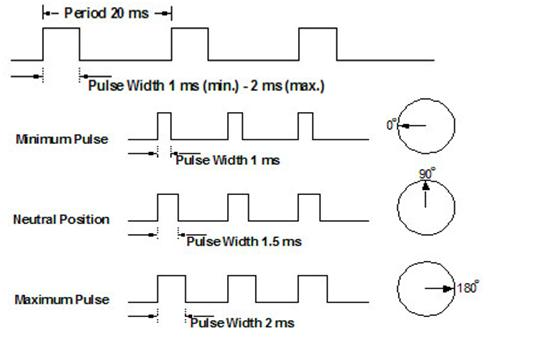
\includegraphics[width=0.8\textwidth]{img/pwm_servo.jpg}
\caption{PWM-servo kontrollsignal \cite{PWM}}
\label{fig:PWM}
\end{figure}   

\subsubsection{Gyrometer}

Et gyrometer er en innretning for å kunne måle vinkelposisjoner i forhold til en fast retning. Gyrometer brukes i mange sammenhenger og finnes i mange varianter, men i denne rapporten vil kun gyrometer av typen MEMS bli beskrevet. 

Et MEMS-gyrometer (Micro Electro-Mechanical System) er lite og lett, og integreres i pakker som likner pakningene til integrerte kretser. Dette gjør at MEMS-gyrometerer enkelt kan legges på kretskort sammen med annen elektronikk. Et MEMS-gyrometer består av en stav, laget i mikromekanikk, ofte formet som en stemmegaffel. Når spenning påføres vil de to tinderene vibrere i motsatt retning av hverandre. Hvis hele staven dreies i en ny retning vil tinderene bli påført motsatt rettetkraft, kapasitansen mellom dem vil da endre seg. Denne kapasitansendringen kan måles og det er dermed mulig å detektere om legemet endrer oreientering.\cite{MEMS}

MPU-6050 fra Invensense, som ble brukt i dette prosjektet, er et 6-akset gyrometer og akselerometer som gir ut data digitalt. Det har en innebygd 10-bit ADC og bruker en I2C-buss for å kommunisere med andre enheter.\cite{InSens}

\subsection{Hardware}
For å kunne styre riggen er det nødvendig å ha en datamaskin ombord i flyet. Det finnes en rekke alternativer på dette området, men her vil Arduino og Raspberry Pi bli presentert. Hovedoppgaven til datamaskinen er å få data fra kameraet, og orientere riggen etter disse. I systemspesifikasjonene til Kongsberg gruppen blir det presisert at det allerede finnes en ekstern GPU på LocalHawk som tar av seg bildebehandling, men en også kan tenke seg en løsning hvor all funksjonalitet er samlet på én chip. Datamaskinen må også kunne håndtere flere prosessorer uten at det blir konflikt mellom dem.

\subsubsection{Arduino}
Arduino er en open source utviklingsplatform basert på \textit{ATmega328}, en 8-bits mikrokontroller. Bruksområdet er hovedsakelig hobbyprosjekter og prototyping. Kortet har 14 digtale porter og 6 analoge inn-porter, som vist i figur \ref{fig:Arduino}. Seks av de digitale portene kan sende PWM-signaler. Siden servomotorer bruker disse signalene er det mulig å koble opp til 6 servomotorer til en Arduino. 

\begin{figure}[h!]
\centering
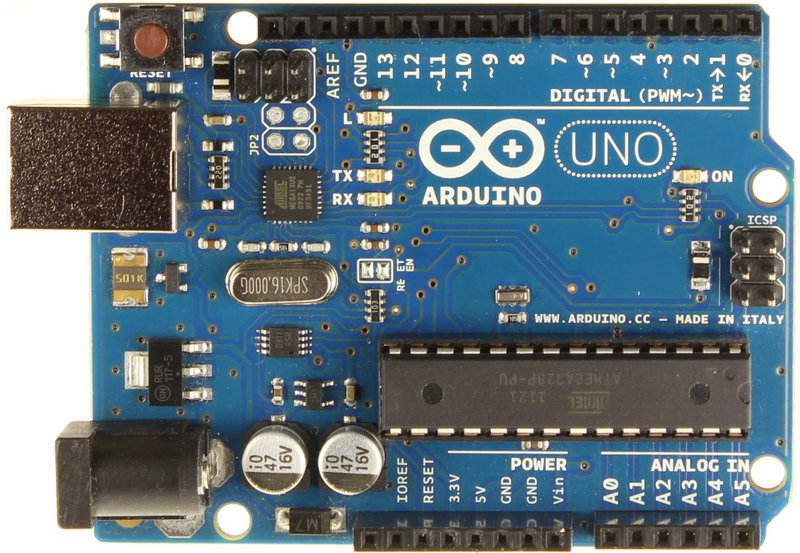
\includegraphics[scale = 0.25]{img/arduinoBoard.jpg}
\caption{Arduino Uno R3 \cite{Arduino}}
\label{fig:Arduino}
\end{figure}

Arduino programmeres i C++, og programmene overføres til kortet via USB. USB-porten på kortet kan også benyttes som COM-port, slik at Arduinoen kan ta inn eksterne kommandoer. Disse kommandoene kan for eksempel være vinkler som en servomotor skal innstilles til. På mikrokontrolleren er det også installert en \textcolor{red}{bootloader som inneholder en rekke biblioteker som gjør at abstraksjonsnivået blir høyere enn ordinær AVR-programmering.}}\colorbox{yellow}{bedre forklaring} Dataregistre trenger ikke å endres når åpning for en ny funksjon, fordi biblioteket håndterer dette.

\subsubsection{Raspberry Pi}
\label{sec:Pi}
Raspberry Pi er en minidatamaskin basert på en 32-bits ARM-arkitektur. Linux er installert på et SD-kort, og all programmering skjer direkte på Raspberry Pi. Maskinen kan brukes ved å koble den til en monitor via HDMI, eller ved å koble den til Internett via nettverksporten og koble seg til via SSH fra en annen datamaskin. Kortet har 8 I/O-pinner, som kan brukes til seriell kommunikasjon. Den er også utstyrt med 2 USB-porter, slik at en for eksempel kan koble til et kamera. En presentasjon av Raspberry PI er gitt i figur \ref{fig:Raspberryfigur}.

\begin{figure}[h!]
\centering
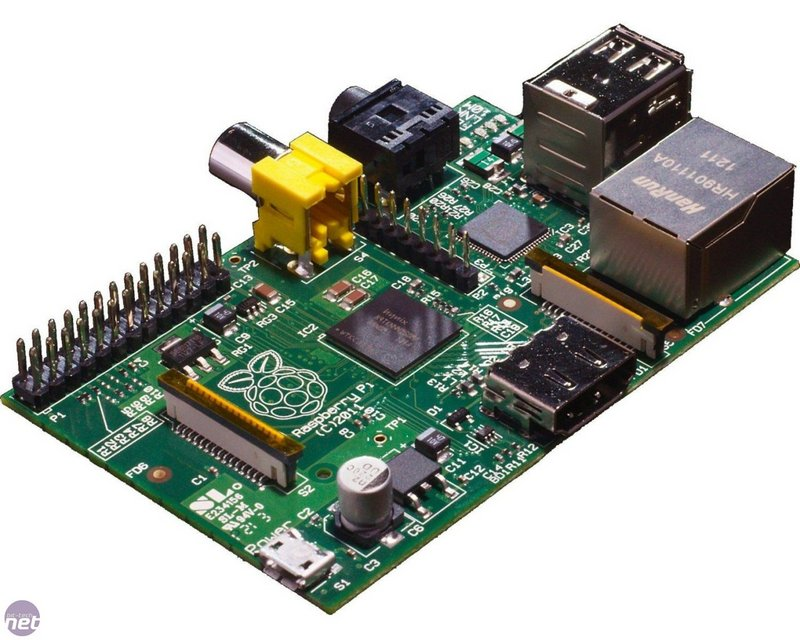
\includegraphics[scale = 0.25]{img/pi.jpg}
\caption{Raspberry Pi Model B \cite{Raspberry}}
\label{fig:Raspberryfigur}
\end{figure}  

\subsubsection{Sammenligning mellom Arduino og Raspberry Pi}
En sammenlikning mellom Arduino Uno og Raspberry Pi model B er gitt i tabell [\ref{tab:ArdRas}]

\begin{table}[H]
\caption{Sammenligning mellom Arduino og Raspberry Pi \cite{ArduinoSpec,RpiSpec}}
\centering
\begin{tabular}{ |c |c |c| }
	\hline
   & Arduino & Raspberry Pi \\
	\hline
  	CPU & 	ATmega328 & ARM1176JZF-S \\
  	Klokkehastighet & 16 MHz & 700 MHz \\
	Minne & 32KB & 512MB\\ 
	CPU-størrelse & 8bit & 32bit\\
	I/O-porter & 14 & 8 \\
	PWN-porter & 6 & 1 \\
	USB-porter & 1 & 2 \\
	Strømforbruk & 250mW & 3.5W\\
	Pris & \$26 & \$35 \\
	\hline  
\end{tabular}
	\label{tab:ArdRas}
\end{table}

Med tanke på spesifikasjoner er Raspberry Pi mye kraftigere enn Arduino Uno med klart raskere prossesor og mye mer minne. En annen fordel er at Raspberry Pi inneholder en GPU, noe Arduino Uno ikke gjør. Dette betyr at Raspberry Pi potensielt kan utføre bildegjenkjenning og styre servoene samtidig. På den andre siden har Raspberry Pi kun én PWM-port, noe som betyr at hvis denne skal styre servoer må to I/O-porter implementeres som PWM-porter i software. Dette vil resultere i mer programmeringsarbeid. En annen ulempe med Raspberry Pi i forhold til Arduino er strømforbruket som er 140\% høyere ved stand-by.\cite{ArduinoSpec,RpiSpec} Kongsberg Gruppen påpeker også at de vil sende opp en egen GPU i flyet, som betyr at bildegjennkjenningen kan gjøres i flyet. Med dette i tankene falt valget på Arduino Uno for å kontrollere servoene.

\subsubsection{Kommunikasjonsprotokoll}

Som nevnt kan det sendes kommandoer til Arduino kortet serielt gjennom en serieport, som også kalles en UART. Det finnes to slike serieporter på Arduino-kortet, og disse er USB-porten og I/O-port 0 (RX) og 1 (TX). I dette prosjektet vil USB-porten bli benyttet for å kommunisere mellom en datamaskin og Arduinokortet. Fordelen med å bruke USB-porten er at det er enkelt, at alle nye datamaskiner har en USB-port og det er ikke nødvendig å lage en egen protokoll med \emph{header}, \emph{error correction} og så videre. En ulempe er at denne protokollen er standard slik at den ikke kan endres for å passe kun dette prosjektet og på denne måten minke mengde \emph{overhead}.

\subsection{Software}

\subsubsection{Matlab, OpenCV og mexopencv}
Matlab brukes til å utforme matematiske modeller, utføre komplekse beregninger og visualisere data. \cite{matlab} Programmet er mye brukt i vitenskapelige miljøer og er meget anerkjent. 
OpenCV er et softwarebibliotek med åpen kildekode som brukes til digital bildebehandling. Biblioteket i versjon 2.x, som er versjonen benyttet i dette prosjektet, og er programmert i C++. \cite{docs:opencv}

For å kunne bruke funksjoner fra OpenCV i Matlab måtte mexopencv tas i bruk. Matlab er ikke uten videre kompatibelt med OpenCV, da dette er programmert i C++. Mexopencv tilbyr Matlabfunksjoner som bygger på flere hundre APIer fra OpenCV. \cite{mexopencv} Dette tillater å programmere alt i Matlab, uten å måtte fokusere på hvordan OpenCV er bygget opp. 
{\thispagestyle{fancy} % All pages have headers and footer}
\newpage
\section{Implementasjon}
\subsection{Bildegjenkjenning}

Vi ble anbefalt å bruke OpenCV av Kongsberg, et open source softwarebibliotek som brukes til bearbeiding av bilder og video. I tillegg til bruken av OpenCV ble vi oppfordret til å bruke Matlab for å programmere. Noen på gruppa hadde erfaringer i Matlab fra før, så vi betraktet ikke dette som noe stort problem.

For å bruke Matlab og OpenCV sammen trengte vi et annet open source prosjekt som het ``mexopencv''. Vi forsøkte en stund å få dette til å fungere, men vi hadde problemer med å sette opp C++, OpenCV og Matlab på en slik måte at mexopencv kunne bruke alle disse ressursene. Noe som førte til ekstra problemer var at de som hadde ansvaret for å begynne med programmeringen satt på to ulike operativsystemer og dermed opplevde forskjellige feilmeldinger underveis. 

Til slutt valgte vi å gå for en løsning hvor vi ikke brukte Matlab. Dette førte til at vi raskt kunne komme igang med utviklingen av bildegjenkjenning og hadde en enkel løsning oppe i løpet av noen dager.

\subsubsection{Første steg}

Den første implementasjonen av gjenkjenningen baserte seg på å konvertere en frame av videoen fra det normale fargespekteret RGB, se figur [\ref{fig:firstiterationrgb}], til et fargespektrum som het HSV\footnote{Hue, Saturation and Value} som vist i figur [\ref{fig:firstiterationhsv}].

\begin{figure}[h!]
	\centering
	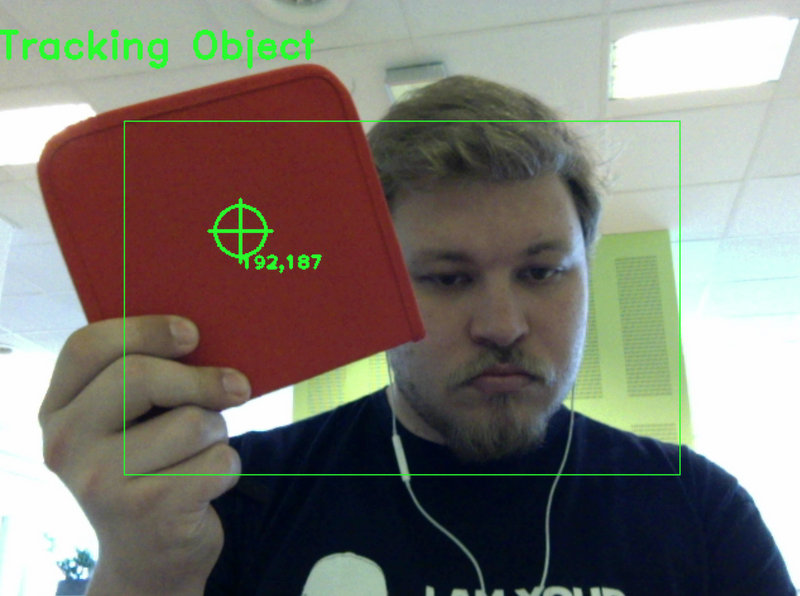
\includegraphics[scale=0.45]{img/first-rgb.jpg}
	\caption[Første iterasjon RGB bilde]{Bilde fra video i vanlig RGB}
	\label{fig:firstiterationrgb}
\end{figure}

\begin{figure}[h!]
	\centering
	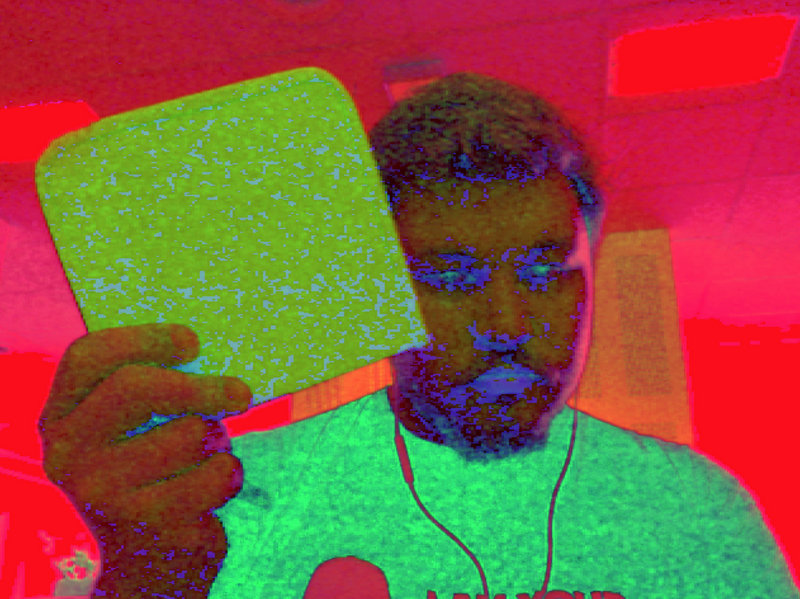
\includegraphics[scale=0.45]{img/first-hsv.jpg}
	\caption[Første iterasjon HSV bilde]{Bilde fra video oversatt til HSV}
	\label{fig:firstiterationhsv}
\end{figure}

HSV baserer seg ikke på blandingen av farger, men bruker nyanser, metningsgrad og lysverdier for å vise en farge . Matrisen med fargekoder som skapes av konverteringen til HSV fører til en skarpere kontrast mellom farger, og gjør jobben med å filtrere vekk uønskede elementer lettere. Vi behandlet deretter matrisen med et filter, som vi manuelt stilte inn med maksimum- og minimumverdier for henholdsvis Hue, Saturation og Value, vist i figur [\ref{fig:sliders}]. Etter at matrisen hadde passert gjennom filteret satt vi igjen med et binært bilde, der fargene som passerte gjennom filteret er gjengitt som hvitt, mens alle andre farger er svarte slik det er vist i figur [\ref{fig:firstiterationbinary}].

\begin{figure}[h!]
	\centering
	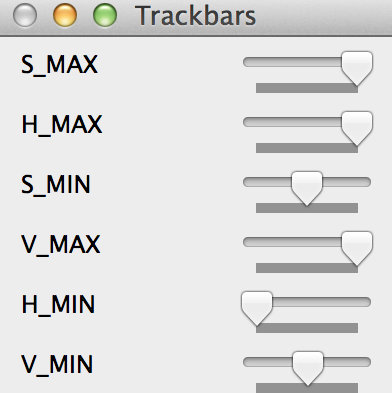
\includegraphics[scale=0.45]{img/sliders.jpg}
	\caption[First iteration HSV image]{Frame from video cast to HSV}
	\caption{Slidere for å velge HSV verdier}
	\label{fig:sliders}
\end{figure}

\begin{figure}[h!]
	\centering
	
\includegraphics[scale=0.45]{img/first-binary.jpg}
	\caption[Første iterasjon binært bilde]{Resultatet av filtrering av et HSV bilde før smoothing}
	\label{fig:firstiterationbinary}
\end{figure}

\subsubsection{Andre steg}

I det første steget klarte vi å fange opp et objekt, men som man kan se i figur [\ref{fig:firstiterationbinary}] er det mye støy i bildet. Vi implementerte derfor en smoothingalgoritme som gikk over det binære bildet og fjernet mindre ansamlinger med punkter og fremhevet de som var større. Dette førte til at vi fikk et renere bilde, med færre og tydeligere objekter. Dette gjorde det betydelig lettere å fange opp de enkelte objektene i bildet og finne det største av dem.

Resultatet kan man se i figur [\ref{fig:seconditerationbinary}] 

\begin{figure}[h!]
	\centering
	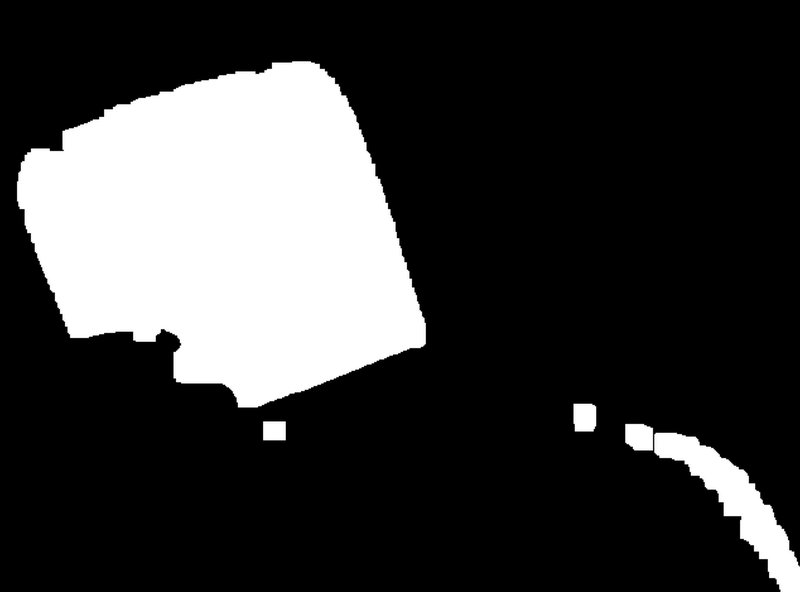
\includegraphics[scale=0.45]{img/second-binary.jpg}
	\caption[Andre iterasjon binært bilde]{Resultatet av filtrering av et HSV bilde etter smoothing}
	\label{fig:seconditerationbinary}
\end{figure}

\subsubsection{Tredje steg}

Etter at vi hadde jobbet en del med systemet fant vi ut at det var tungvindt å stille inn verdiene som skulle følges hver gang. Løsningen ble da at vi implementerte et enkelt kommandogrensesnitt som kunne be programmet om å følge etter fargen som befant seg i sentrum av bildet, som vist i figur [\ref{fig:commandmenu}]

\begin{figure}[h!]
	\centering
	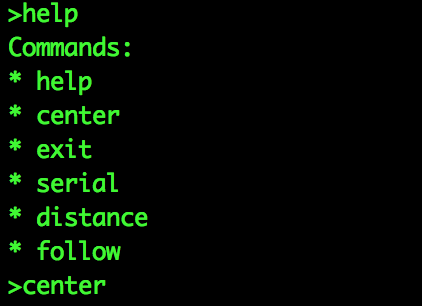
\includegraphics[scale=0.8]{img/command-menu.png}
	\caption{Kommandomenyen}
	\label{fig:commandmenu}
\end{figure}

\subsection{Konstruksjon av riggen}

\subsubsection{Planlegging}
Riggens oppgave er å endre synsretningen til kameraet etter kommando fra bildegjennkjenningen. Synsvinkelen kan modeleres som en vektor, hvor retningen til vektoren er variabel. Hvis vektoren, $\bf{v}$, settes inn i et koordinatsystem med utspring i origo og sfæriske koordinater, kan situasjonen beskrives som i figur [\ref{fig:spher}]

\begin{figure}[h!]
	\centering
	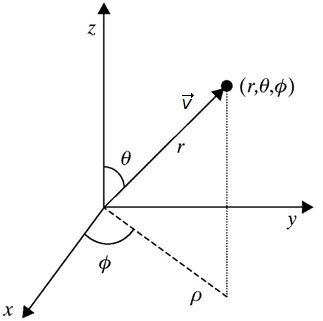
\includegraphics[scale=0.5]{img/RettVek.jpg}
	\caption{Sfærisk koordinatsystem}
	\label{fig:spher}
\end{figure}

hvor $\phi$ er vinkelen mellom x- og y-aksene og $\theta$ er vinkelen mellom z-aksen og xy-planet. Siden riggen skal festes til et fly og kameraet skal se ned på bakken vil det ikke være behov for vinkelretningen å bevege seg inn i den øvre halvdelen av koordinatsystemet. Det betyr at $\phi$ og $\theta$ kun trenger 180 graders utsving for å dekke hele den nedre halvdelen. Dermed kan hele dette omerådet dekkes ved hjelp av to servomotorer med 180 graders utslag satt sammen som i figur [\ref{fig:IdeRigg}]. 

\begin{figure}[h!]
	\centering
	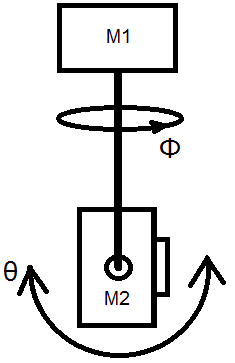
\includegraphics[scale=0.5]{img/BasicRiggIde.png}
	\caption{Servostyring av $\theta$ og $\phi$}
	\label{fig:IdeRigg}
\end{figure}

Hvor kameraet festes til servomotor 2 som beveger seg i retning $\theta$, mens servomotor 1 beverger servo2 og kamera i retning $\phi$. For å kunne trekke riggen inn i flyet ved landing ble det bestemt å feste riggen på en bom som kunne heves å senkes ved hjelp av en servomotor som vist i figur [\ref{fig:bom}].

\begin{figure}[h!]
	\centering
	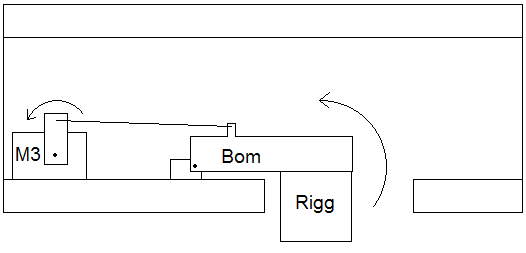
\includegraphics[scale=0.5]{img/Motor3.png}
	\caption{Servomotor 3 kan heve riggen inn i flykroppen.}
	\label{fig:bom}
\end{figure}


\subsubsection{Sammenstilling}
Riggen ble sammenstilt med målene på prototypeflyet til kongsberg som utgangspunkt [\ref{ref:PowerPoint}]. Med disse målene ble det klart at servomotorene måtte være små i størrelse og valget falt på servomotoren HD-1600A. Med sine beskjedene fysiske mål på 21.3x11.6x22.8 mm og en vekt på 6g [\ref{ref:PowerHD}], ble HD-1600A ansett som perfekt for dette formålet. HS-50 fra Hitec ble også vurdert, men med lavere dreimoment og betydelig høyere pris ble HD-1600A regnet som et bedre alternativ. For å bygge delene som skulle koble servoene sammen ble det brukt 6mm MDF plater fordi disse er stive og relativt sterke. Dette fører til at de ikke bøyes eller gir etter ved raske rotasjoner. Figur [\ref{fig:RiggTegn}] viser hvordan servomotorene er koblet sammen og figur [\ref{fig:RiggBilde}] viser et bilde av den ferdige prototype riggen. 

\begin{figure}[h!]
	\centering
	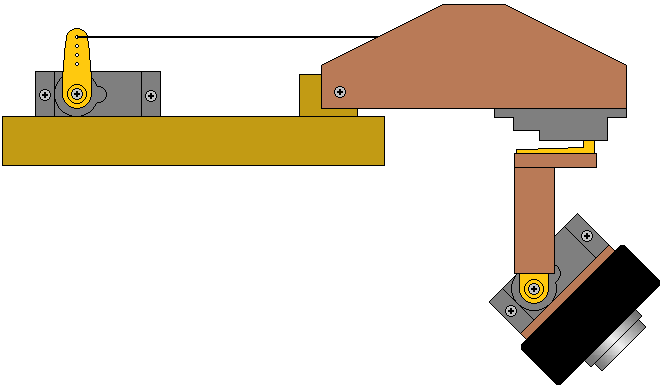
\includegraphics[scale=0.5]{img/RIGG_sattsammen.png}
	\caption{Tegning av mekaniske rigg}
	\label{fig:RiggTegn}
\end{figure}

Servomotorene styres av et PWM signal som genereres av en Arduino UNO. Biblioteket $Servo.lib$ brukes for å kontrollere servoene gjennom tre I/O porter. Servo 1 er koblet til port 9, servo 2 er koblet til port 6 og servo 3 er koblet til port 3. Siden det viste seg ved målinger at hver servo, under last, kan trekke opp mot 250mA, ble det valgt å bruke en ekstern 6V batteripakke, med fire seriekoblede 1.5V AA batterier, koblet inn som vist i figur [\ref{fig:ArduSkjem}]. Dette isteden for å la servoene trekke forsyningsstrøm rett fra 5V pinnen til arduinokortet. Arduinokortet bruker strøm fra USB og denne kan ikke levere mer enn 500mA ,på grunn av innebygget sikring i Arduino. Dermed kan ikke Arduinokortet levere de ca. 750mA som trengs dersom alle servoene går med stor last samtidig. 

\begin{figure}[h!]
	\centering
	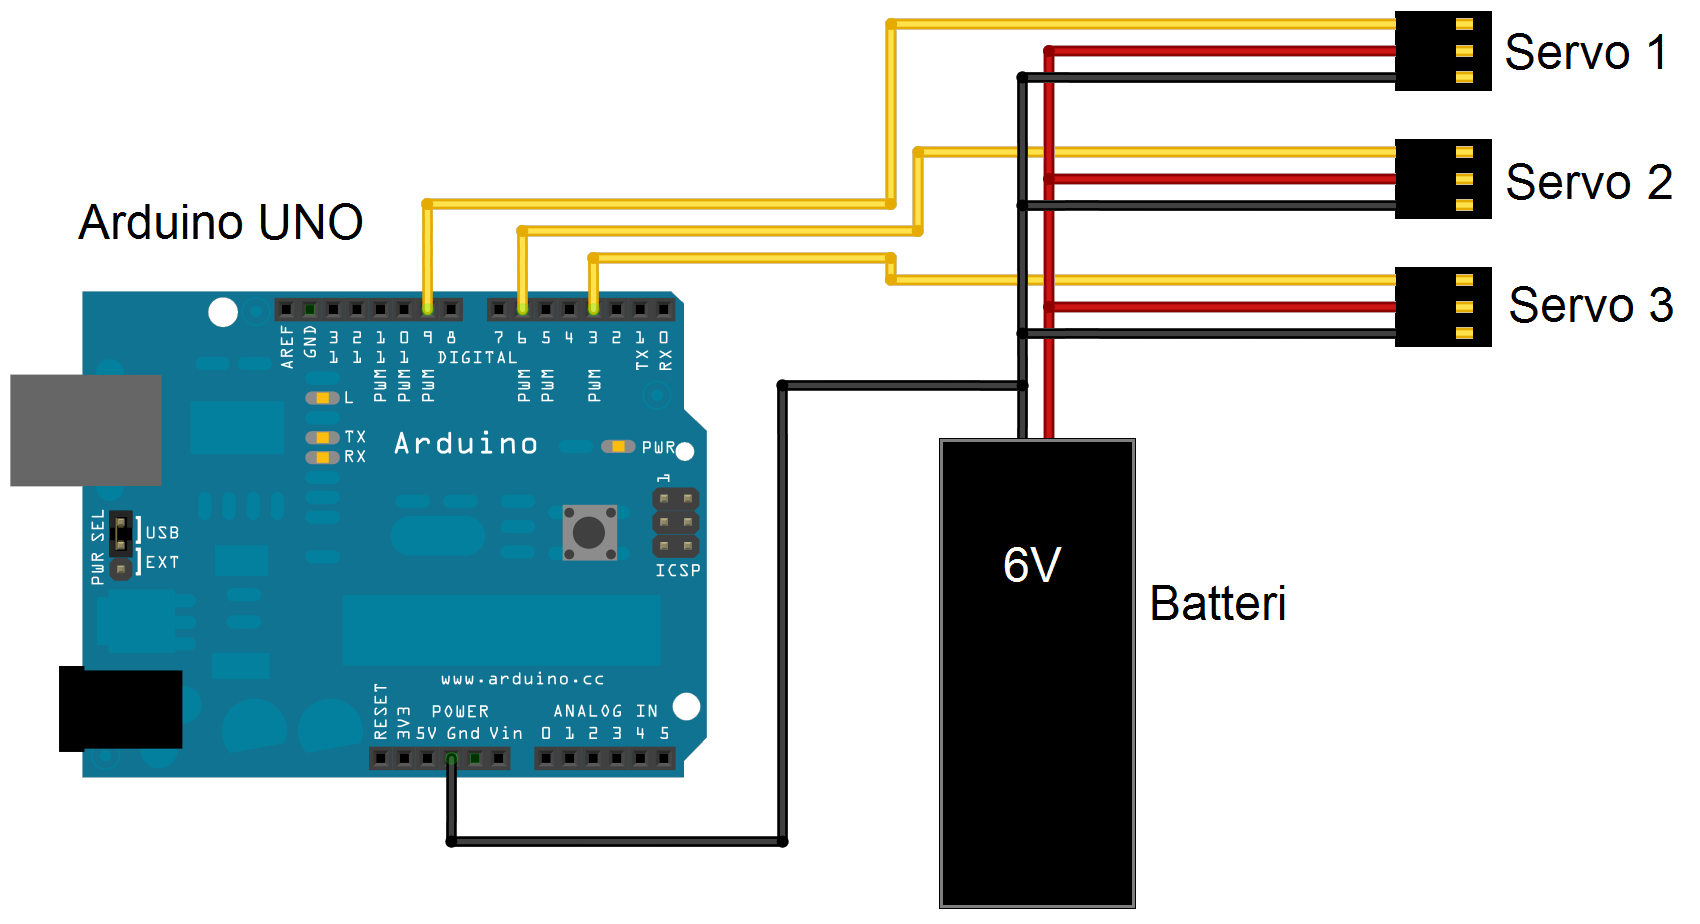
\includegraphics[scale=0.25]{img/KoblingsskjemaArduino.png}
	\caption{Koblingsskjema for Arduino}
	\label{fig:ArduSkjem}
\end{figure}  

Kommandoer sendes til Arduino via USB porten. Kommandoer kan sendes som $Char$ på formen ``100a120b40c'', hvor tallene foran``c'' forteller posisjon til servo 1, tallene for ``b'' gir posisjon til servo 2 og tallene foran ``c'' posisjonenen til servo 3. Dermed vil strengen ``100a120b40c'' flytte servo 1 til 100 grader, servo 2 til 120 grader og servo 3 til 40 grader. De gyldige vinklene er fra 0 til 180 grader. Hvis ``200'' sendes vil servo 1 stoppe på 180 grader. 


\subsection{Styring av rigg + bildegjenkjenning}

Tekst her{\thispagestyle{fancy} % All pages have headers and footer}
\newpage
\section{Diskusjon}
--- Setninger hentet ut fra implementasjon som egentlig er diskusjon ---: Dette må legges til på riktig plass i diskusjon. Viktig!
\begin{itemize}
\item Kongsberg gruppen ble informert om dette, og de var enige i at det var en god løsning. -> Opencv <-
\item igang med utviklingen og innen få dager hadde vi utviklet en enkel løsning for bildegjenkjenning.
\tem Som konsekvens av å ha skiftet språk til C++, hadde utviklingen raskt fremtog. 

\end {itemize}
--- Setninger hentet ut fra implementasjon som egentlig er diskusjon ---

\begin{itemize}
\item 
Hva kunne vært fordelen med å gå over til Raspberry PI med sine servoer

\item diskutere kompleksiteten ved bildegjenkjenning. 

\item diskutere behandling av bilder i flyet med egen gpu

\item diskutere utfordringene med å følge bilen med flyet, med tanke på svingene på banen og flyets krenging.

\item hva de neste steg i prosessen blir, for å komme frem til et brukbart produkt. 
\end{itemize}

\subsection{Implementasjonen}
 
\subsubsection{Mekanisk installasjon}

Kameraet som ble brukt var et billig 300K piksels webkamera. Dette til tross for at Kongsberg sendte et kamera som var tiltenkt brukt i LokalHawk flyet. Riggen ble i utgangspunktet bygget for et mindre kamera, og Kongsberg sitt var for stort og tungt for konstruksjonen. Det ble vurdert å bygge ny rigg, men valget falt på å skaffe et mindre og billigere kamera. 

På grunn av liten tid til testing mot slutten av prosjektet ble også servomotor 3 benyttet til å følge objekter selvom denne egentlig bare skulle brukes til å heve å senke riggen. Dette fordi det var enklere å implemnetere en algoritme for å følge objekt med 3 servoer. Det viste seg at servo 3 kunne vibrere så lenge bommen ``hvilte'' på armen til denne. Det var bare en liten vibrasjon, men den kan ha innvirkning hvis objektet er langt fra kameraet og bildet er zoomet inn. Denne vibrasjonen er nok mest sannsynlig på grunn av oppdateringshastigheten til servoen. Som nevnt tidligere er denne på 50Hz og vibrasjonen kunne vært enda mindre ved bruk av digitale servoer som har høyere oppdateringshastighet.  

\subsubsection{Gyrometer}
Gyrometeret i systemet skulle bli benyttet til å simulere flyets krengninger. Det kunne da bli demostrert hvordan riggen ville oppføre seg mens den var i bevegelse. Drivere til gyrometeret fantes ferdig til Arduino, og det var få problemer å få det til å virke. Det oppsto derimot problemer da servoene skulle implimenteres i samme program. Det ble konflikt mellom de to bibliotekene fordi begge benytter seg av samme timer på Arduinoen. Siden det ikke er multithreading på Arduino, er det ikke mulig å få et synkront program. Gyro-biblioteket fungerte også bra til Raspberry Pi. Gyrometeret ble valgt bort da det var problematisk å få servoene til å virke på Raspbery Pi. En løsning med en enkelt Arduino og tre servoer servoer ble derfor benyttet. 

For systemets helhet, er ikke gyrometeret vital. I spesifikasjonene til Kongsberg blir det presisert at systemet allerede inneholder et gyrometer. Ved en fullstending implementasjon vil kan denne bli brukt. Et eget gyrometer resulterer i et system som er uavhengig av den eksisterende hardwaren på Local Hawk. Dette medfører at systemet blir lettere overførbart til andre plattformer.

\subsubsection{Bildegjenkjenning}

Det tok ikke veldig lang tid før det måtte erkjennes at bildegjenkjenningen var mye mer utfordrende enn først antatt. Selv en oppgave som å følge et ensfarget objekt medfører ganske komplekse algoritmer. Små endringer i lysforhold kan være nok til å endre kvaliteten på et bilde nok til at objektet plutselig faller gjennom filteret i programmet eller at forstyrrende elementer fra bakgrunnen kommer gjennom filteret og fører til en mengde støy som gjør at programmet ikke finner noe klart objekt å forfølge.

Målet for bildegjenkjenningen var å klare å følge meget komplekse objekter i varierende terreng. En bil brukt i bilsport vil ofte ha en eller flere farger som grunnfarge, i tillegg har vil det være et udefinert antall klistremerker og påmalte kjennemerker som annonser, navn og annet. I utviklingen av algoritmene ble det aldri tid til å komme forbi steget der ensfargede objekter i varierte bakgrunner skal benyttes. Dette fungerte nesten utelukkende dersom kontrasten på fargen til objektet var stor nok i forhold til bakgrunnen til at de enkelt kunne skilles fra hverandre.

Bildebehandling er et komplisert fagfelt, og gjenkjenning av kompliserte objekter, som realistiske biler, er en kompleks prosess som krever lang erfaring og en svært stor mengde arbeid. Arbeid med bildegjenkjenning på det nivået som kreves for å skille ut objekter i graden som ønskes av Kongsberg var ikke mulig å oppnå i den relativt korte tiden som var tilgjengelig for dette prosjektet.

\subsubsection{Ressursbruk i bildegjenkjenning og bruk i flyet}

Bildegjenkjenning er en tung prosess som krever noe hardware for å utføre operasjonen fortløpende. En relativt kraftig CPU trengs når videostrømmen skal behandles i sanntid. I spesifikasjonene fra Kongsberg \cite{LocalHawkPDF} var det ikke spesifisert noen form for hardware som støtter den mengden prosessering som er nødvendig for gjenkjenningen. I samtaler med Kongsberg kom det frem at de vurderte å utstyre flyet med en egen GPU for å utføre bildegjenkjenning. 

GPU har i nyere tid kommet til en formfaktor og energibruk som egner seg godt til bruk for et prosjekt som dette. OpenCV har egne pakker som inkluderer støtte for bruk av GPU for behandling av bilder, og kodebasen som er utviklet i dette prosjektet kan derfor i stor grad benyttes selv om denne løsningen blir brukt.

\subsubsection{Nedskalering av oppgaven}
Arbeidet med prosjektet kom fort igang, oppgaven var tidlig valgt ut og teknologiene som skulle benyttes bestemt. Bildegjenkjenningen hadde vanskeligheter i begynnelsen, særlig med biblioteket \emph{mexopencv}. Problemer med installasjon førte resulterte i at programmeringen aldri var på et stadie der vi kunne begynne å bruke Matlab. Det tok noen uker med forsøk før vi bestemte oss for å bytte til C++, som programmeringsspråk etter en samtale med Kongsberg.

Rundt tiden da samarbeidsavtalen ble revidert ble det klart at gruppa ikke kunne komme i mål med hele oppgaven slik den var fremstilt av Kongsberg. Prosjektets tilstand ble diskutert innad i gruppen, og i samråd med faglærer ble en prototype av bildestabiliseringsriggen bestemt til å være en bedre proporsjonert oppgave for den gitte tidsrammen.

\subsection{Videre arbeid}
Siden prototyperiggen presentert i denne oppgaven er for liten til å bære kameraet Konsberg ønsker å bruke i sitt LocalHawk, er en naturlig videre føring av dette prosjektet å bygge en ny rigg og forbedret rigg med større servoer og materialer mer egent vær og vind. Det neste steget vil kunne være å bruke et gyrometer, som det ble forsøkt i dette prosjektet, til å stabilisere denne riggen slik at den blir mest mulig uavhengig av flyets bevegelser. 

Bildegjenkjenningen trenger fremdeles en god del arbeid før den kan brukes i faktiske forhold. Som tidligere nevnt innebærer dette nesten et selvstendig prosjekt hvor fokuset er på bearbeidingen av bilder og integrasjon av denne teknologien mot en innebygget GPU i flyet. Prototypen som er utviklet i dette prosjektet viser tydelig hvordan oppgaven med bildestabilisering kan løses som en isolert oppgave. Resultatet tar ikke for seg hvordan bilens endrede kjøreretning vil påvirke flyets krengning, og deretter hvordan dette dekkes av kameraet.

Kongsberg så for seg en løsningen som et hyllevareprodukt som kan plasseres under flyet. En videreføring av implementasjonen vil være å lage et eget kretskort med gyro, CPU og GPU. Til dette formålet kan ARM-prosessor benyttes, som også har innebygget GPU med god ytelse. Et felt som ikke blir dekket i denne rapporten er signaloverføringen fra flyet og til en bakkestasjon. Til dette formålet kan WiFi eller GSM-nettet bli benyttet. Et moment som må bli tatt hensyn til, er at mange tilskuere på banen kan påvirke signaloverføringen.

Beslutningen om nedskalering av prosjektet medførte å påvise at riggen i prinsippet klarer å følge etter objekter. I dag er stabiliseringen litt hakkete, noe som bare betyr at det kan gjøres med for å forsøke å enten forutsi hvilken vei objektet sannsynligvis beveger seg eller å la kameraet følge litt etter slik at banen kameraet skal følge kan finstilles mer.

{\thispagestyle{fancy} % All pages have headers and footer}
\newpage
\section{Konklusjon}
Planleggingsfasen av prosjektet var preget av at det ble gjort en litt for optimistisk ved vurdering av hvor mye som var tilgjengelig innenfor rammene av faget. Oppgaven som ble presentert av Kongsberg gruppen hadde mye relevant for faget, samt at det hørtes meget spennende ut. Arbeidet med prosjektet har ført til alle på gruppa har lært mye nytt, både om arbeidet ved ukjente teknologier og kompleksiteten ved disse.

Prototypen som ble laget selekterer ut et objekt fra en videostrøm og deretter dirigerer en mekanisk rigg med et kamera, slik at objektet hele tiden holder seg i sentrum. Prototypen ble bygget opp av tre analoge servoer av typen PowerHD, som benytter seg av PDM-signal for justering av retning. For modellering av bildene ble C++ brukt i kombinasjon med OpenCV, noe som viste seg å fungere utmerket til dette formålet. 

Det gjenstår en del arbeid før det som er påbegynt, kan brukes i sammenheng med flyet som Kongsberg gruppen har sett for seg. Bildegjenkjenning er et komplekst område i seg selv, og egner seg nok som et eget prosjekt uavhengig av om LocalHawk skal inkluderes. I tillegg vil det være fornuftig å benytte seg av for eksempel en Raspberry PI. Dette vil bidra til støtte for multi-threading, noe som igjen gjør det mulig å benytte seg av et for eksempel et gyrometer i tillegg til kamerafeeden.  {\thispagestyle{fancy} % All pages have headers and footer}
\newpage
\colorbox{yellow}{Kildene er lite beskrivende. Kan vi ha et annet system på referansestrukturen?}
\begin{thebibliography}{9}

\bibitem{reference:PWMcontrolPic} \label{ref:PWM} http://www.electroons.com/electroons/servo$\_$control.html
\bibitem{reference:PowerHD} \label{ref:PowerHD} http://www.chd.hk/
\bibitem{reference:ServoCtrl} \label{ref:SerCtrl} http://pcbheaven.com/wikipages/How$\_$RC$\_$Servos$\_$Works/
\bibitem{reference:InvenSense} \label{ref:InSens} http://www.invensense.com/
\bibitem{reference:PowerPoint} \label{ref:PowerPoint} PowerPoint av Konsberg gruppen

\end{thebibliography}{\thispagestyle{fancy} % All pages have headers and footer}

\end{document}
